\documentclass[xetex,mathserif,serif]{beamer}
\usepackage{polyglossia}
\usepackage{minted}
\usepackage{tabu}

\usepackage{textpos}
\setlength{\TPHorizModule}{1cm}
\setlength{\TPVertModule}{1cm}

\useoutertheme{infolines}

\usepackage{fontspec}
\setmainfont{FreeSans}
\newfontfamily{\russianfonttt}{FreeSans}

\setbeamertemplate{blocks}[rounded][shadow=false]
\setbeamercolor*{block title example}{fg=green!50!black,bg=green!20}
\setbeamercolor*{block body example}{fg=black,bg=green!10}

\setbeamercolor*{block title alerted}{fg=red!50!black,bg=red!20}
\setbeamercolor*{block body alerted}{fg=black,bg=red!10}

\definecolor{cadmiumgreen}{rgb}{0.0, 0.42, 0.24}

\tabulinesep=0.7mm

\newcommand{\attribution}[1] {
\vspace{-5mm}\begin{flushright}\begin{scriptsize}\textcolor{gray}{\textcopyright\, #1}\end{scriptsize}\end{flushright}
}

\title{Глубокое метамоделирование}
\author[Юрий Литвинов]{Ю.В. Литвинов \newline 
	\textcolor{gray}{\small\texttt{y.litvinov@spbu.ru}}
}

\date{13.03.2018г}

\begin{document}

	\frame{\titlepage}

	\section{Введение}

	\begin{frame}
		\frametitle{О визуальных языках}
		\begin{itemize}
			\item Модели -- неформальные или формальные
			\item Языки моделирования: UML, IDEFx, BPMN, SDL, ...
			\item Языки визуального программирования: Simulink, LabView, ...
			\item Предметно-ориентированные визуальные языки: TRIK Studio, Robolab, Node-RED, ...
		\end{itemize}
		\begin{center}
			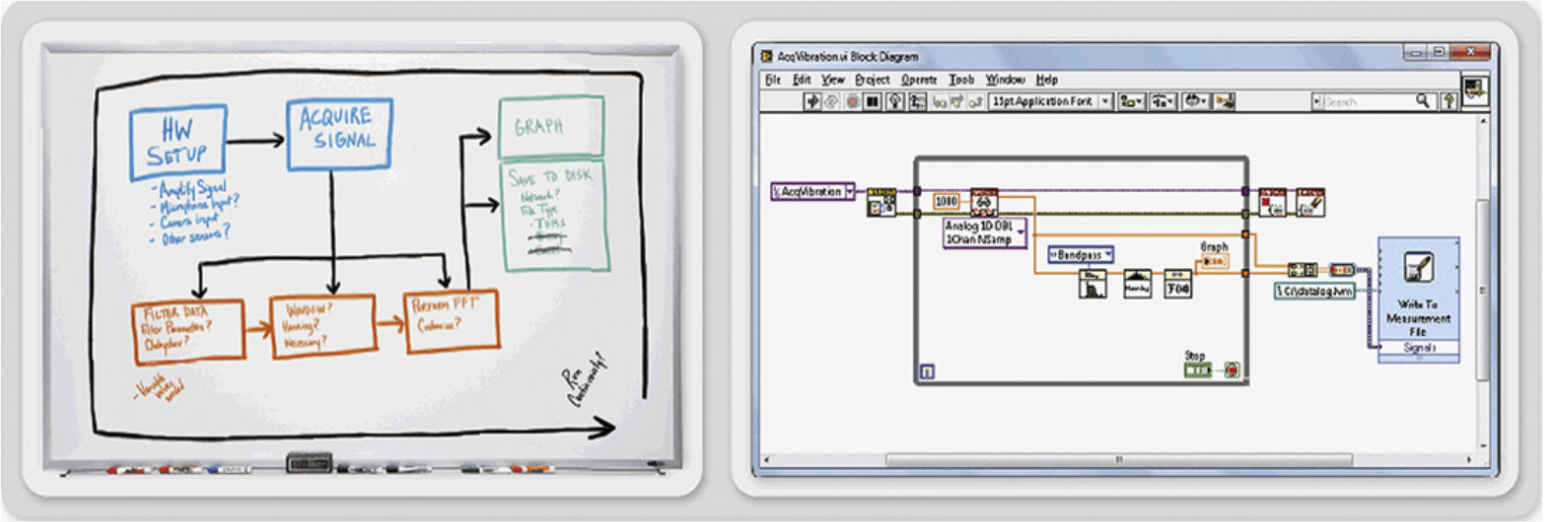
\includegraphics[width=0.8\textwidth]{sketchesVsFormalNotations.png}
			\attribution{N. Medvidovic}
		\end{center}
	\end{frame}

	\begin{frame}
		\frametitle{Язык UML}
		\begin{columns}
			\begin{column}{0.45\textwidth}
				\begin{itemize}
					\item Самый известный визуальный язык
					\item Появился в середине 90-х
					\item Не язык, а набор языков
					\item 14 разных видов диаграмм
					\item Единое описание, общее ``ядро'' языка
					\item Плохо с семантикой
					\item Использует метамоделирование для задания синтаксиса
				\end{itemize}
			\end{column}
			\begin{column}{0.55\textwidth}
				\begin{center}
					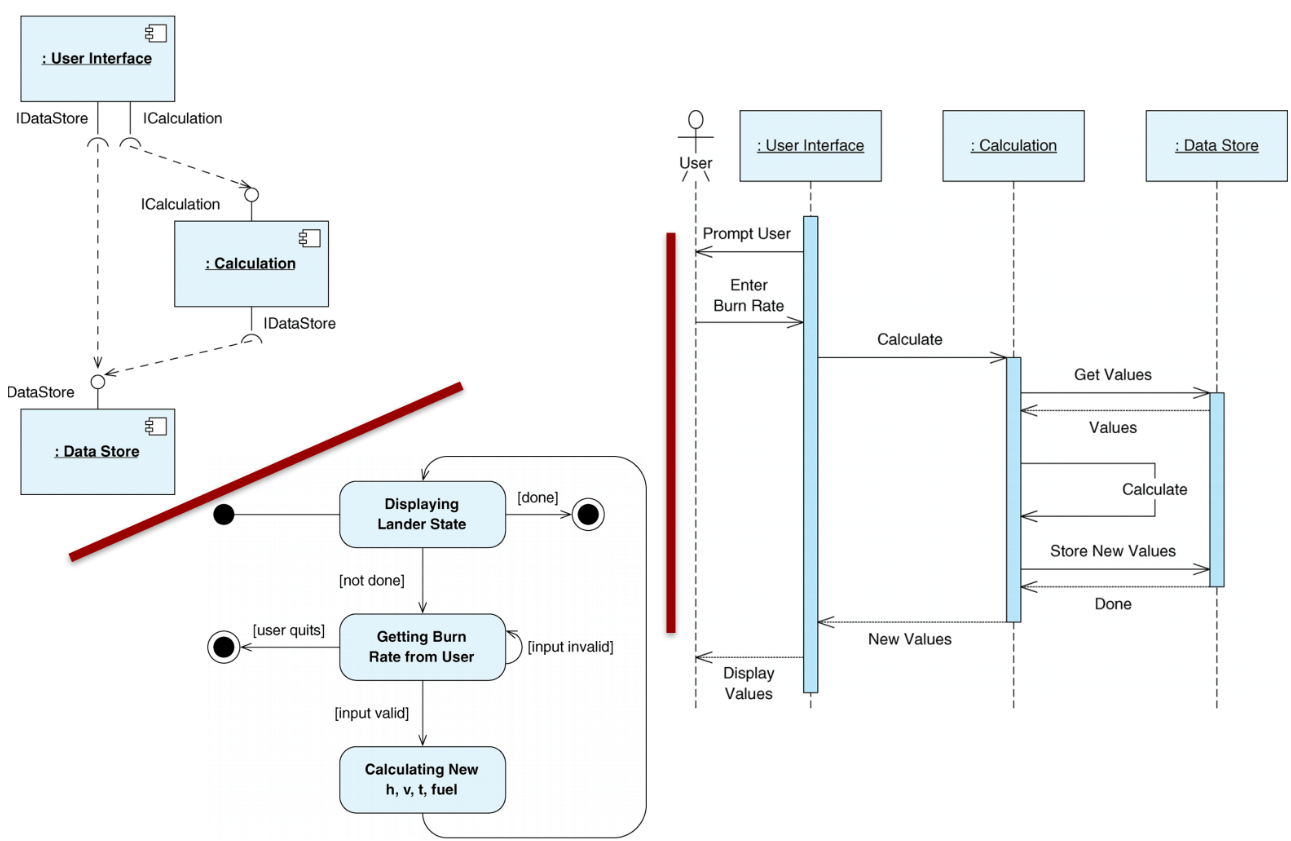
\includegraphics[width=0.8\textwidth]{uml.png}
					
					\vspace{5mm}
					
					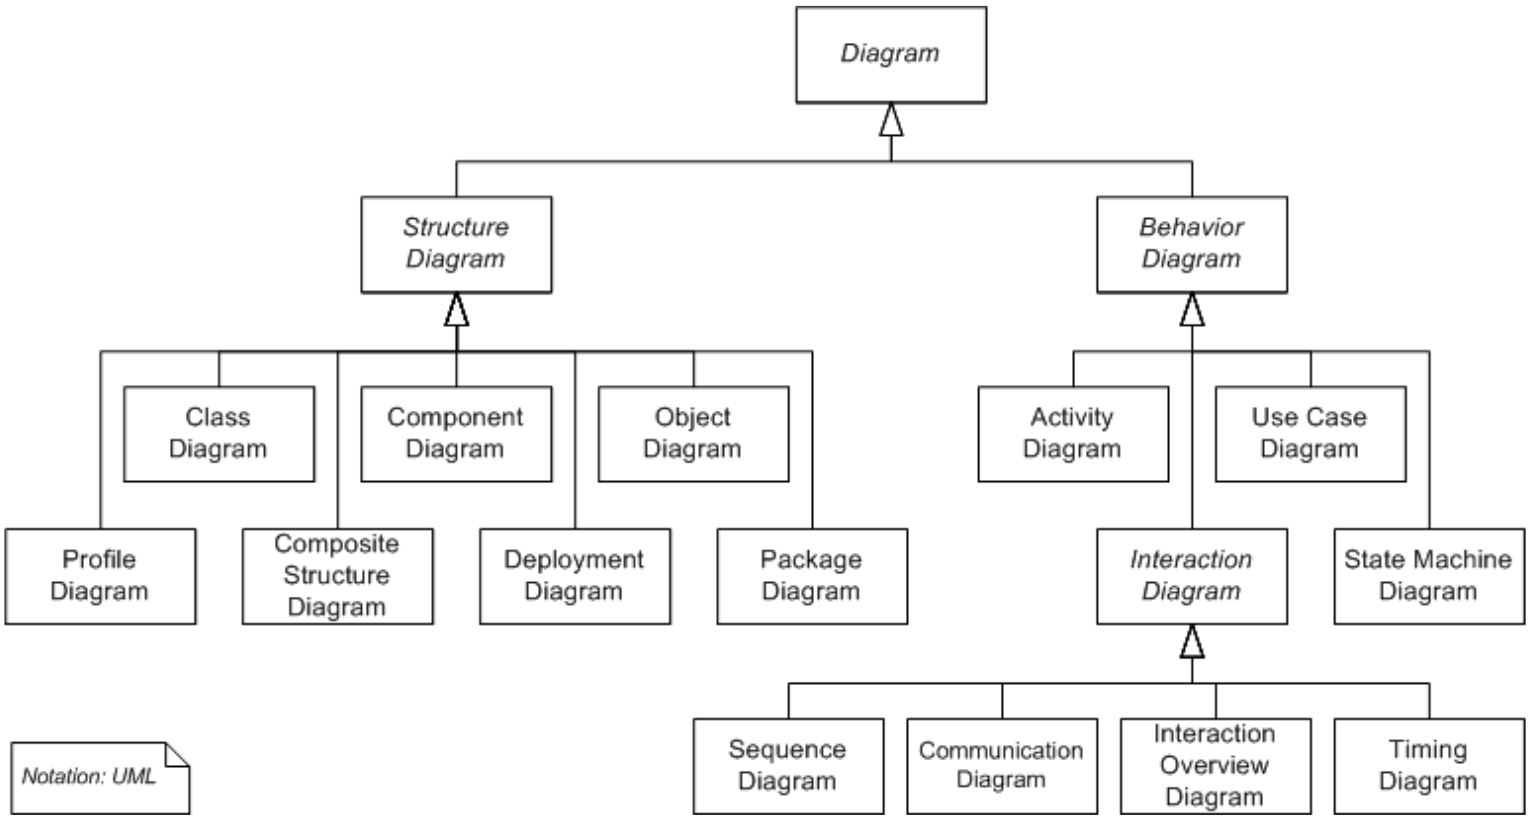
\includegraphics[width=0.8\textwidth]{umlDiagrams.png}
				\end{center}
			\end{column}
		\end{columns}
	\end{frame}

	\begin{frame}
		\frametitle{Метамоделирование}
		\begin{center}
			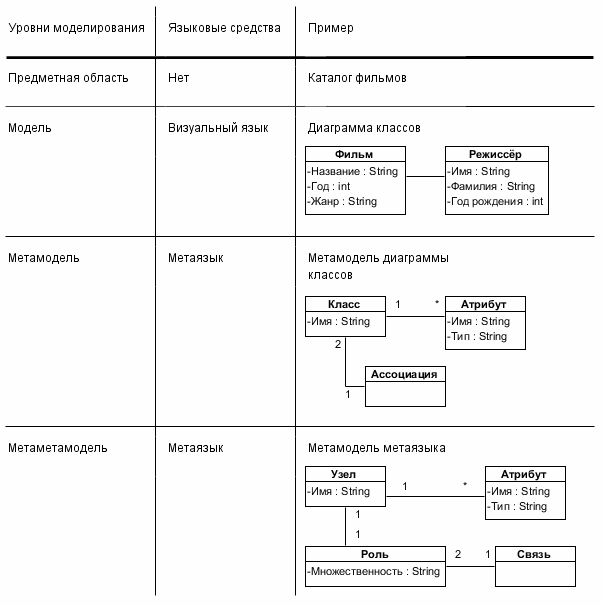
\includegraphics[width=0.6\textwidth]{metalevels.png}
		\end{center}
	\end{frame}

	\section{Проблемы с метамоделью UML}

	\begin{frame}
		\frametitle{Неоднозначность толкования ``instanceOf''}
		\framesubtitle{Пример}
		\begin{center}
			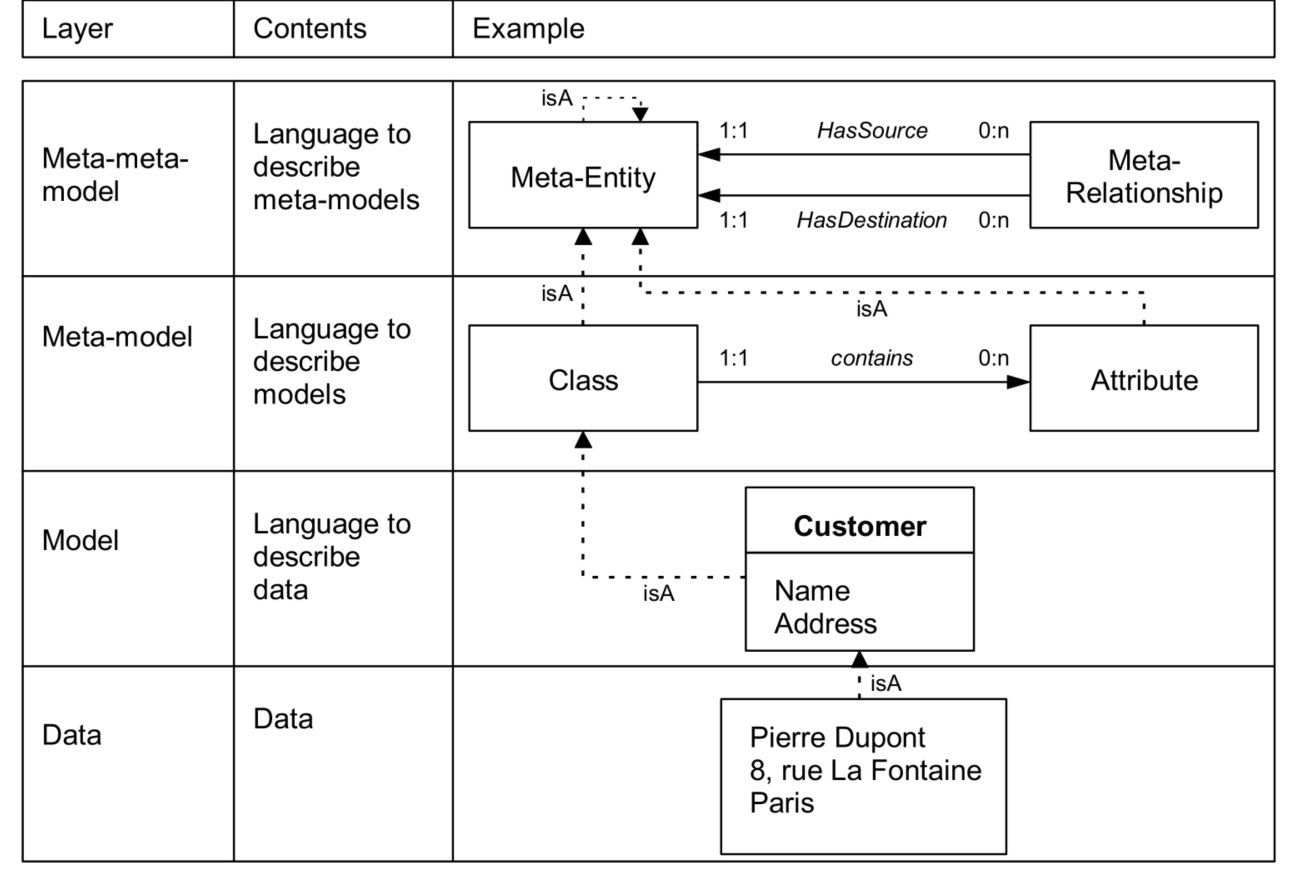
\includegraphics[width=0.7\textwidth]{bezivinExample.png}
			\attribution{J. Bezivin et al., Ontology-Based Layered Semantics for Precise OA\&D Modeling, 1997}
		\end{center}
	\end{frame}

	\begin{frame}
		\frametitle{Неоднозначность толкования ``instanceOf''}
		\framesubtitle{Собственно проблема}
		\begin{center}
			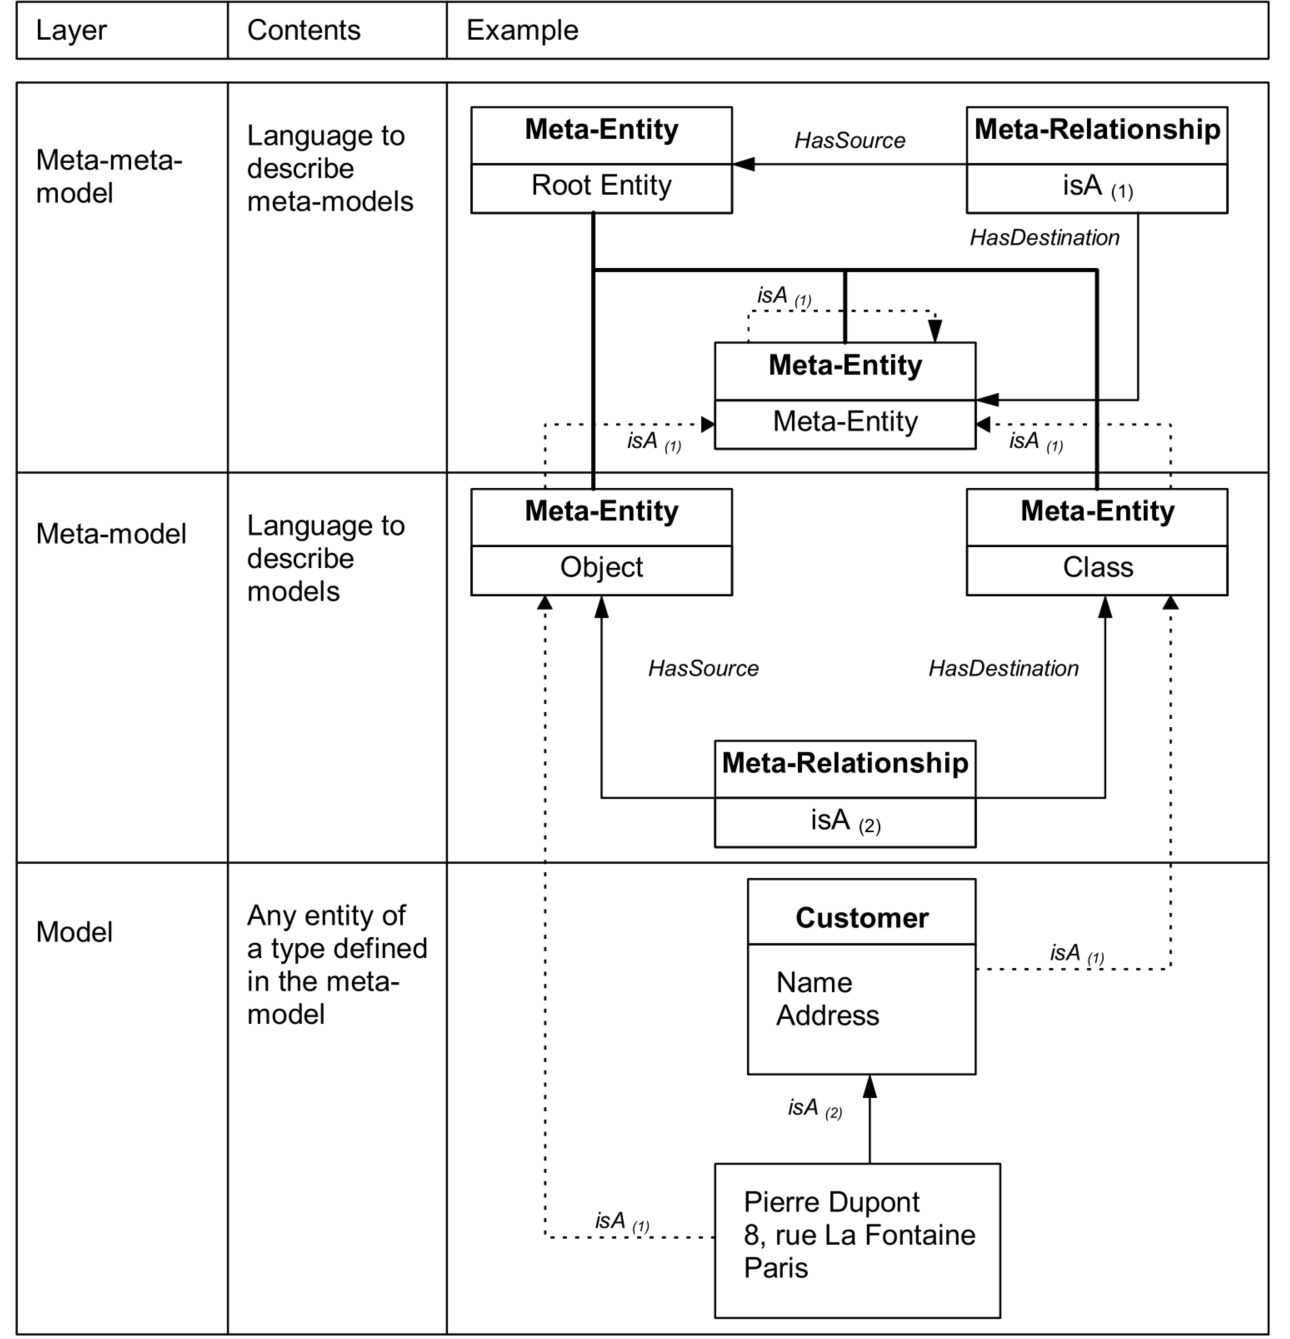
\includegraphics[width=0.55\textwidth]{bezivinIsA.png}
		\end{center}
	\end{frame}

	\begin{frame}
		\frametitle{Ещё один пример}
		\begin{center}
			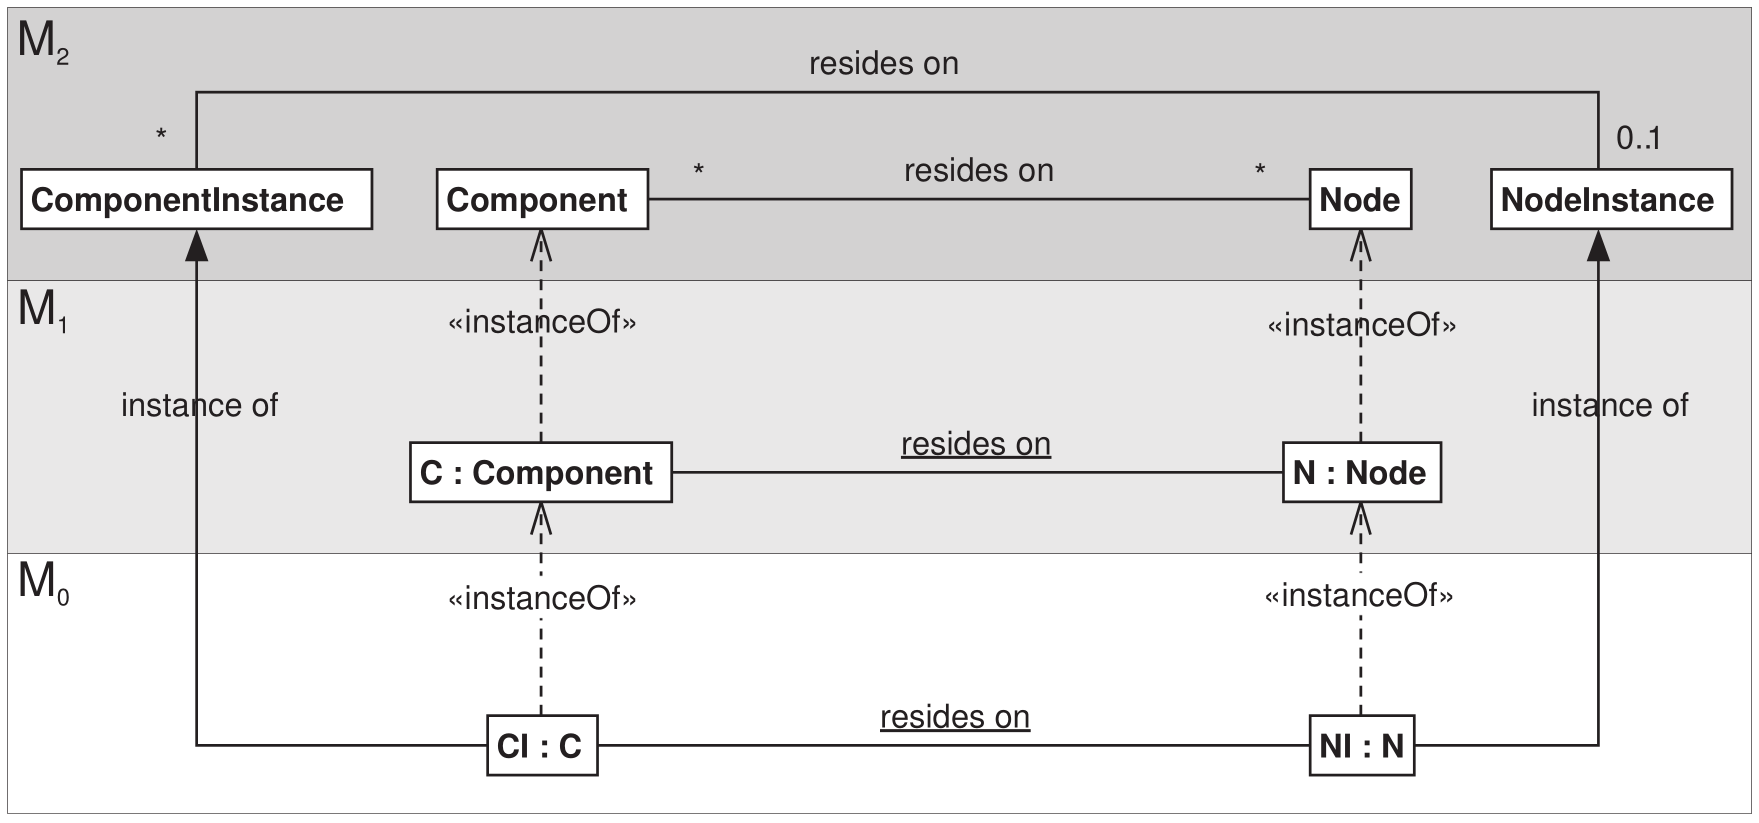
\includegraphics[width=0.8\textwidth]{atkinsonInstanceOf.png}
			\attribution{C. Atkinson, Th. Kuhne, The Essence of Multilevel Metamodeling, 2001}
		\end{center}
	\end{frame}

	\begin{frame}
		\frametitle{Умножение сущностей}
		\begin{center}
			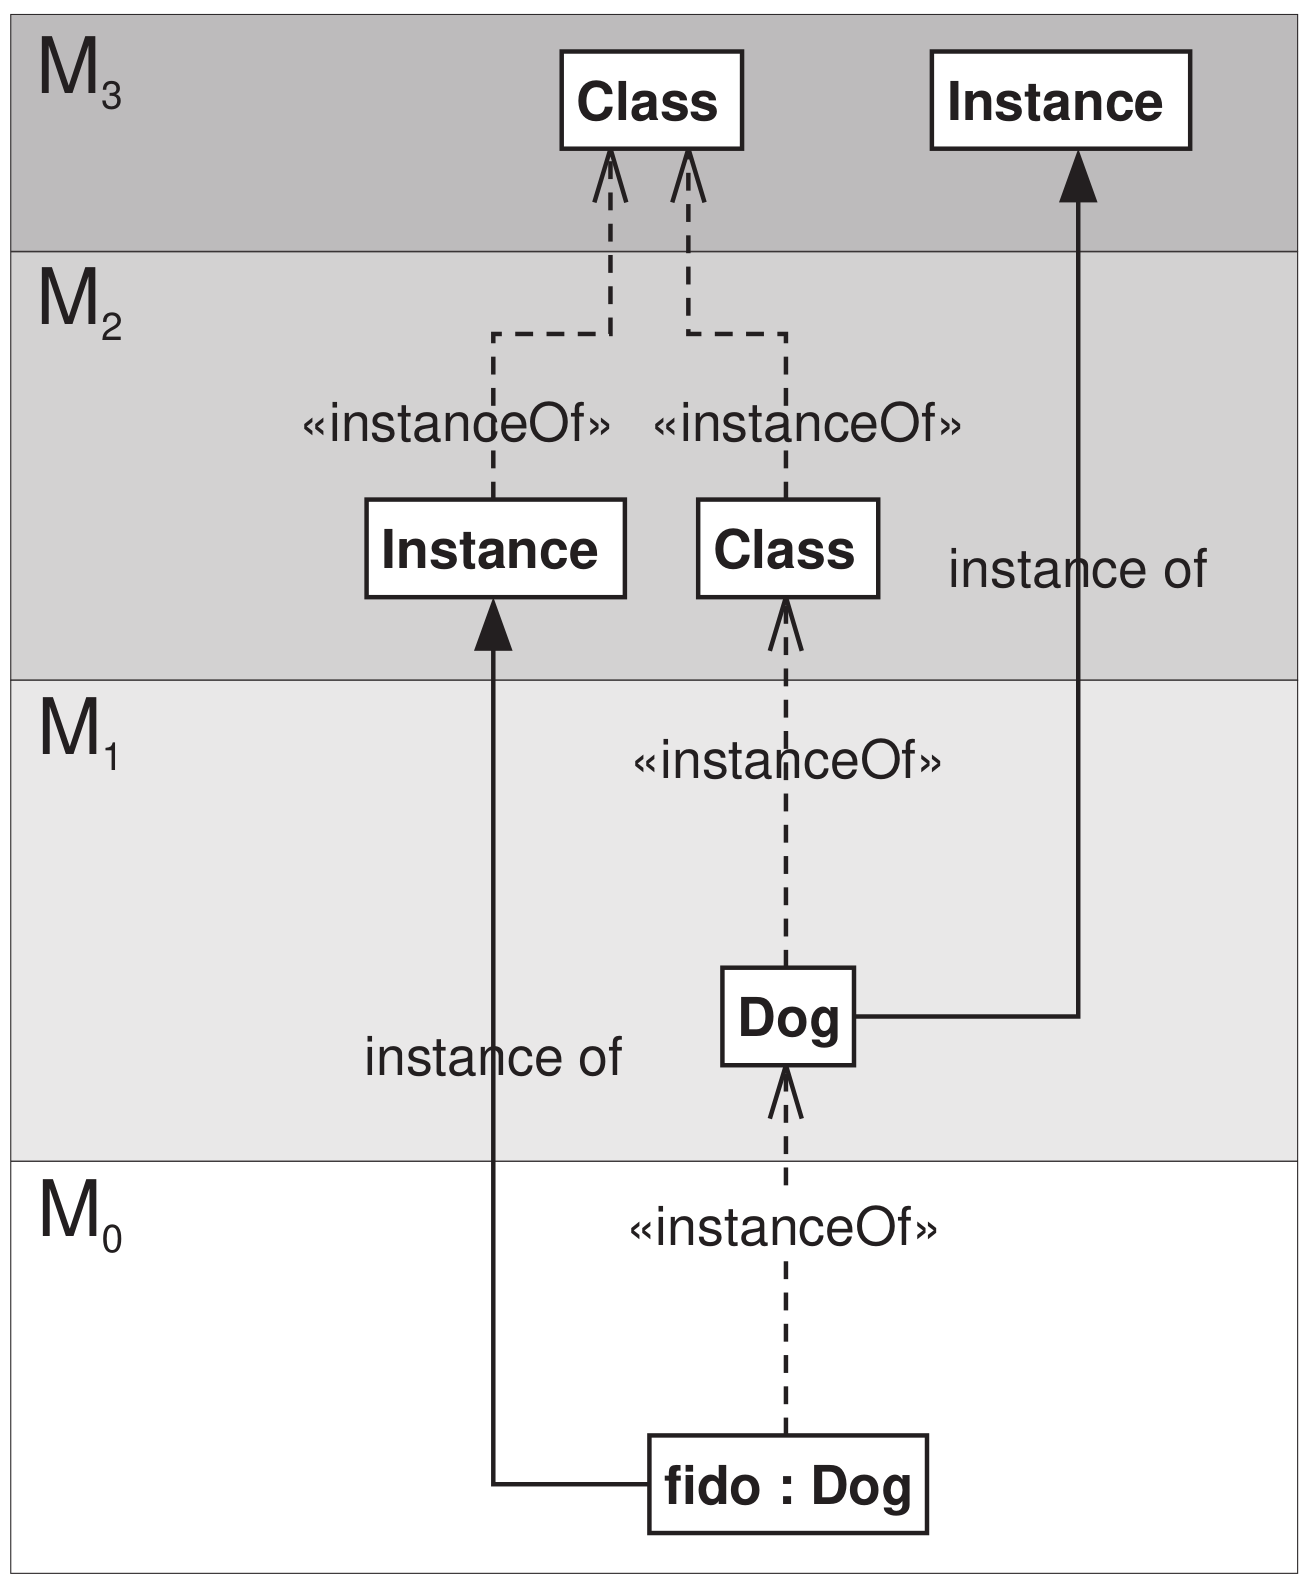
\includegraphics[width=0.45\textwidth]{atkinsonDuplication.png}
			\attribution{C. Atkinson, Th. Kuhne, The Essence of Multilevel Metamodeling, 2001}
		\end{center}
	\end{frame}

	\begin{frame}
		\frametitle{``Пользовательский уровень'', подпрограммы}
		\begin{center}
			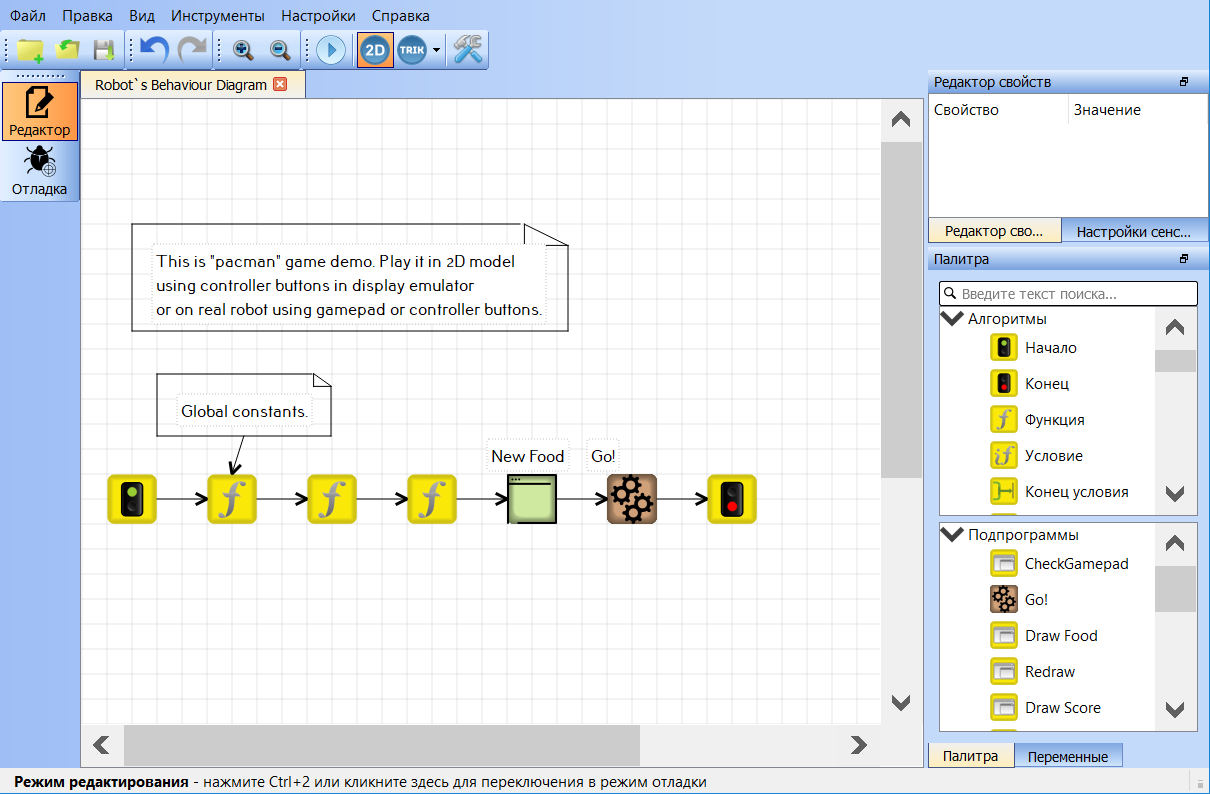
\includegraphics[width=0.90\textwidth]{trikStudio.png}
		\end{center}
	\end{frame}

	\section{Глубокое метамоделирование}

	\begin{frame}
		\frametitle{Глубокое метамоделирование}
		\begin{itemize}
			\item Разрешить метатипам определять структуру элементов на несколько метауровней ниже
			\item \textit{Clabject} --- класс-объект, с атрибутами и полями со значениями
			\item \textit{Potency} --- число, показывающее, на сколько метауровней вниз элемент может быть инстанцирован
			\item \textit{Level} --- метауровень, на котором определён элемент
			\item Инстанцирование применимо только к элементам с $potency > 0$ и уменьшает $potency$ и $level$ на 1
			\item \textit{Dual fields} --- поля, имеющие значение, и могущие быть инстанцированы
			\item \textit{Single fields} --- ``обычные'' поля, принимающие значение, только если их $potency = 0$
		\end{itemize}
	\end{frame}

	\begin{frame}
		\frametitle{Пример}
		\begin{center}
			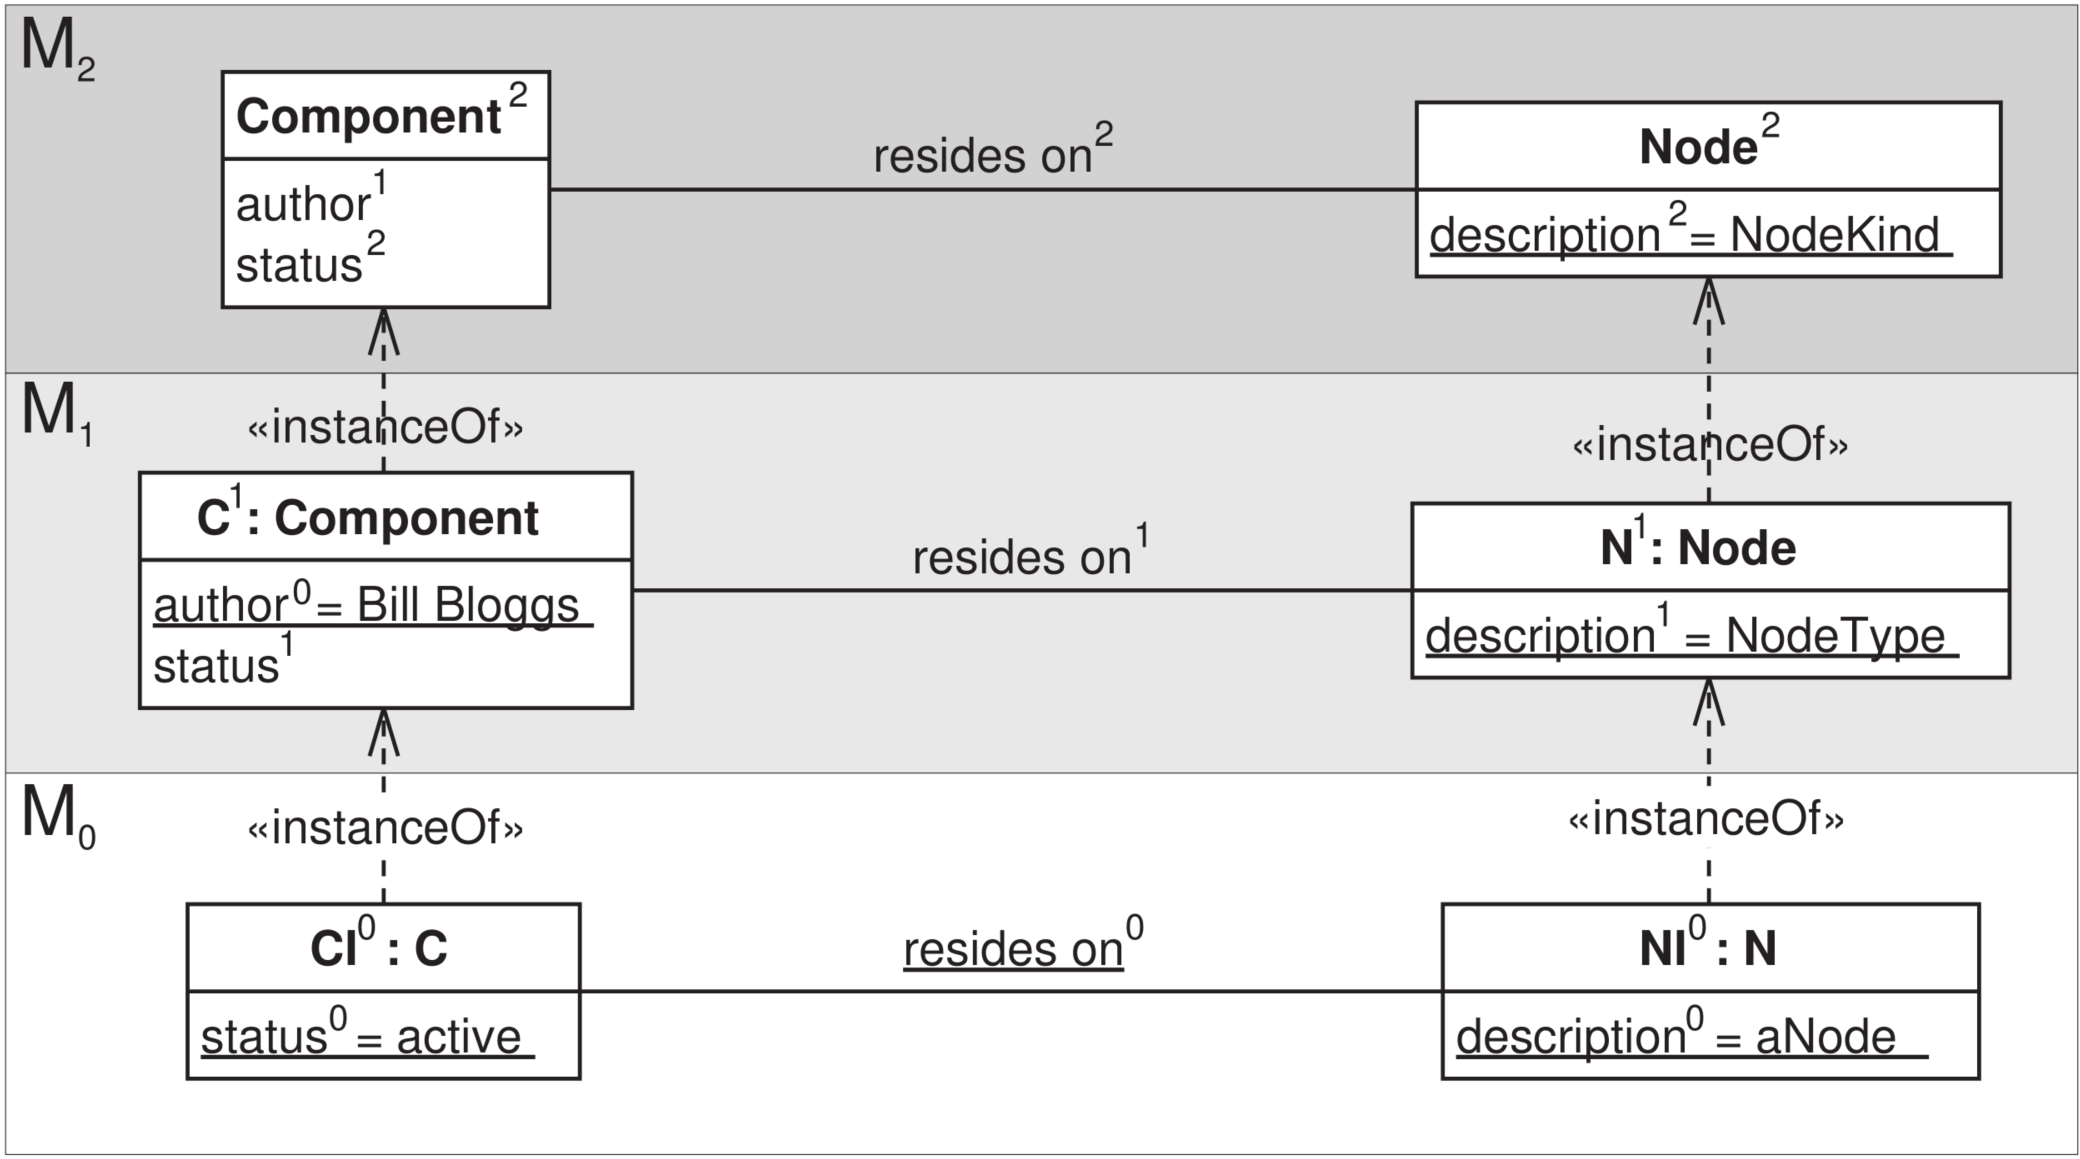
\includegraphics[width=0.8\textwidth]{deepComponents.png}
			\attribution{C. Atkinson, Th. Kuhne, The Essence of Multilevel Metamodeling, 2001}
		\end{center}
	\end{frame}

	\begin{frame}
		\frametitle{Метаметамодель для глубокого метамоделирования}
		\begin{center}
			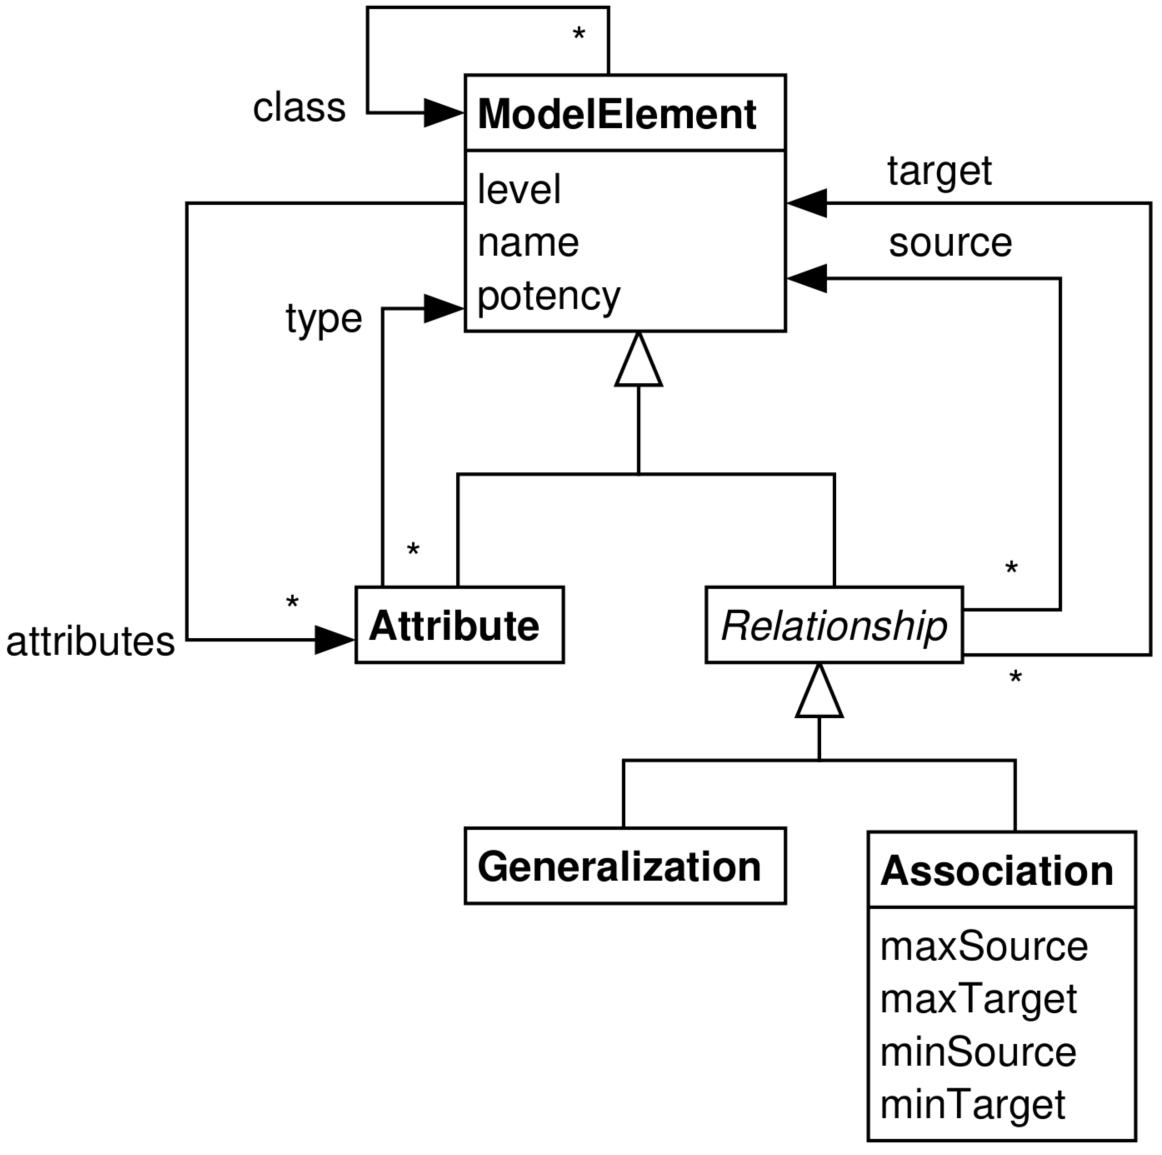
\includegraphics[width=0.5\textwidth]{momm.png}
			\attribution{C. Atkinson, Th. Kuhne, The Essence of Multilevel Metamodeling, 2001}
		\end{center}
	\end{frame}

	\section{Ортогональное метамоделирование}

	\begin{frame}
		\frametitle{Ортогональное метамоделирование}
		\begin{center}
			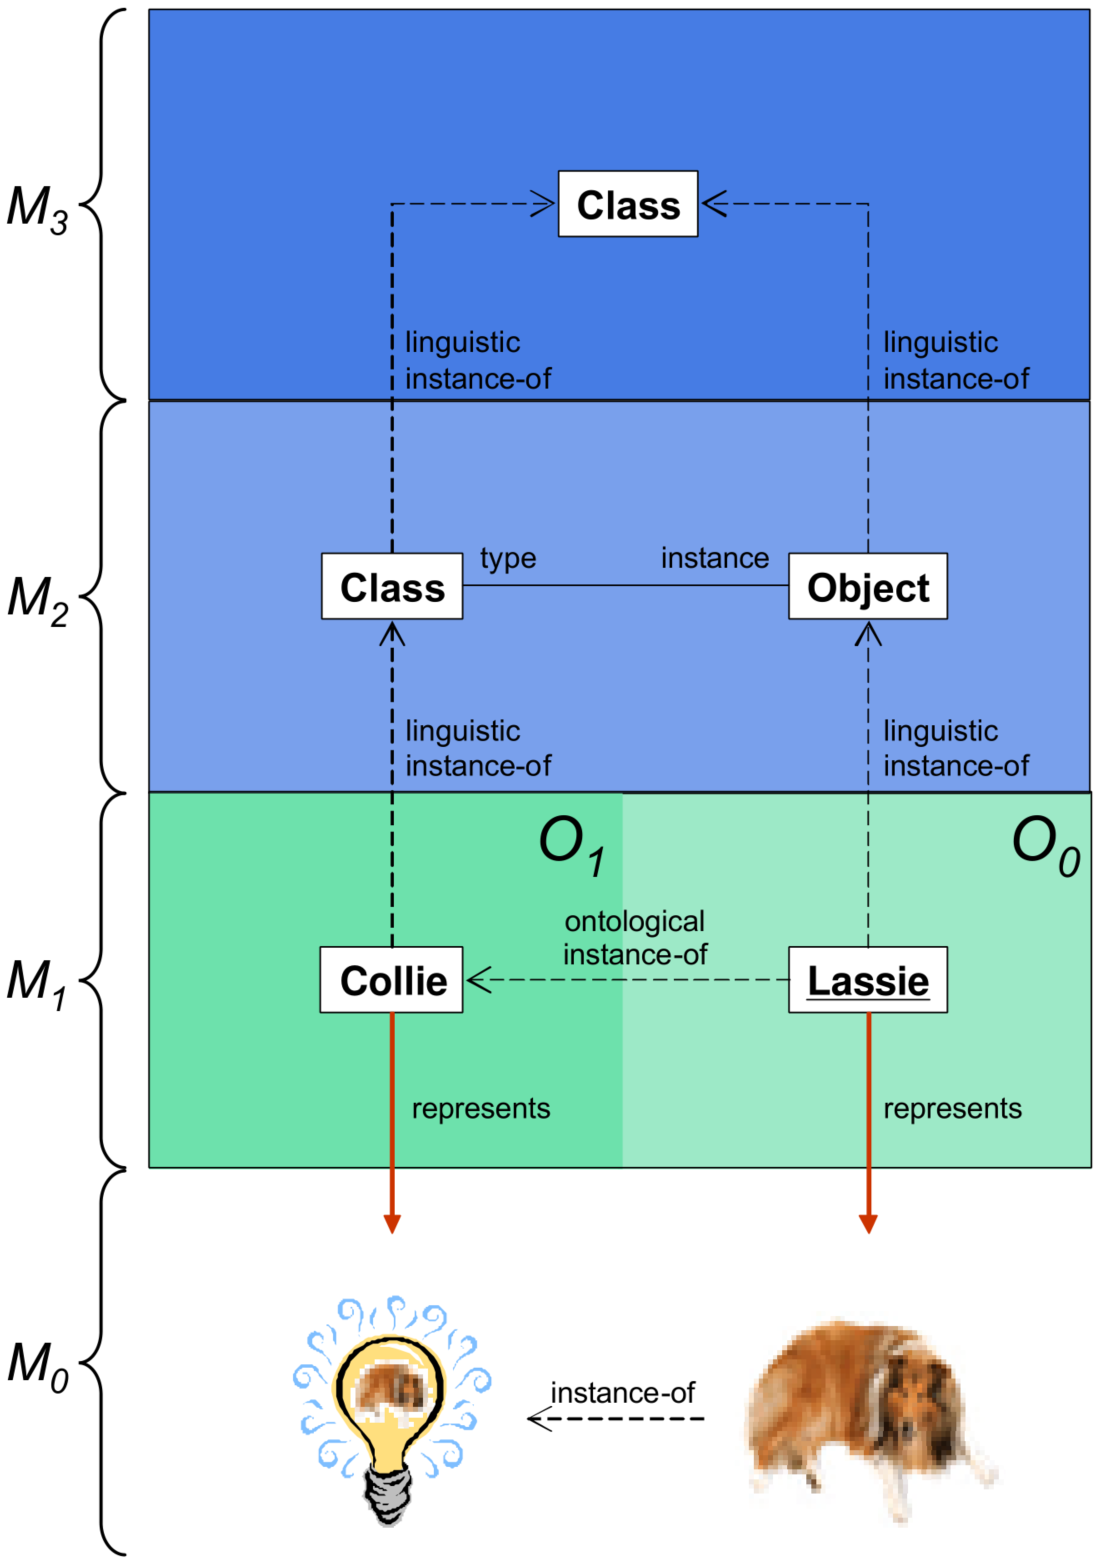
\includegraphics[width=0.35\textwidth]{linguisticView.png}
			\hspace{1cm}
			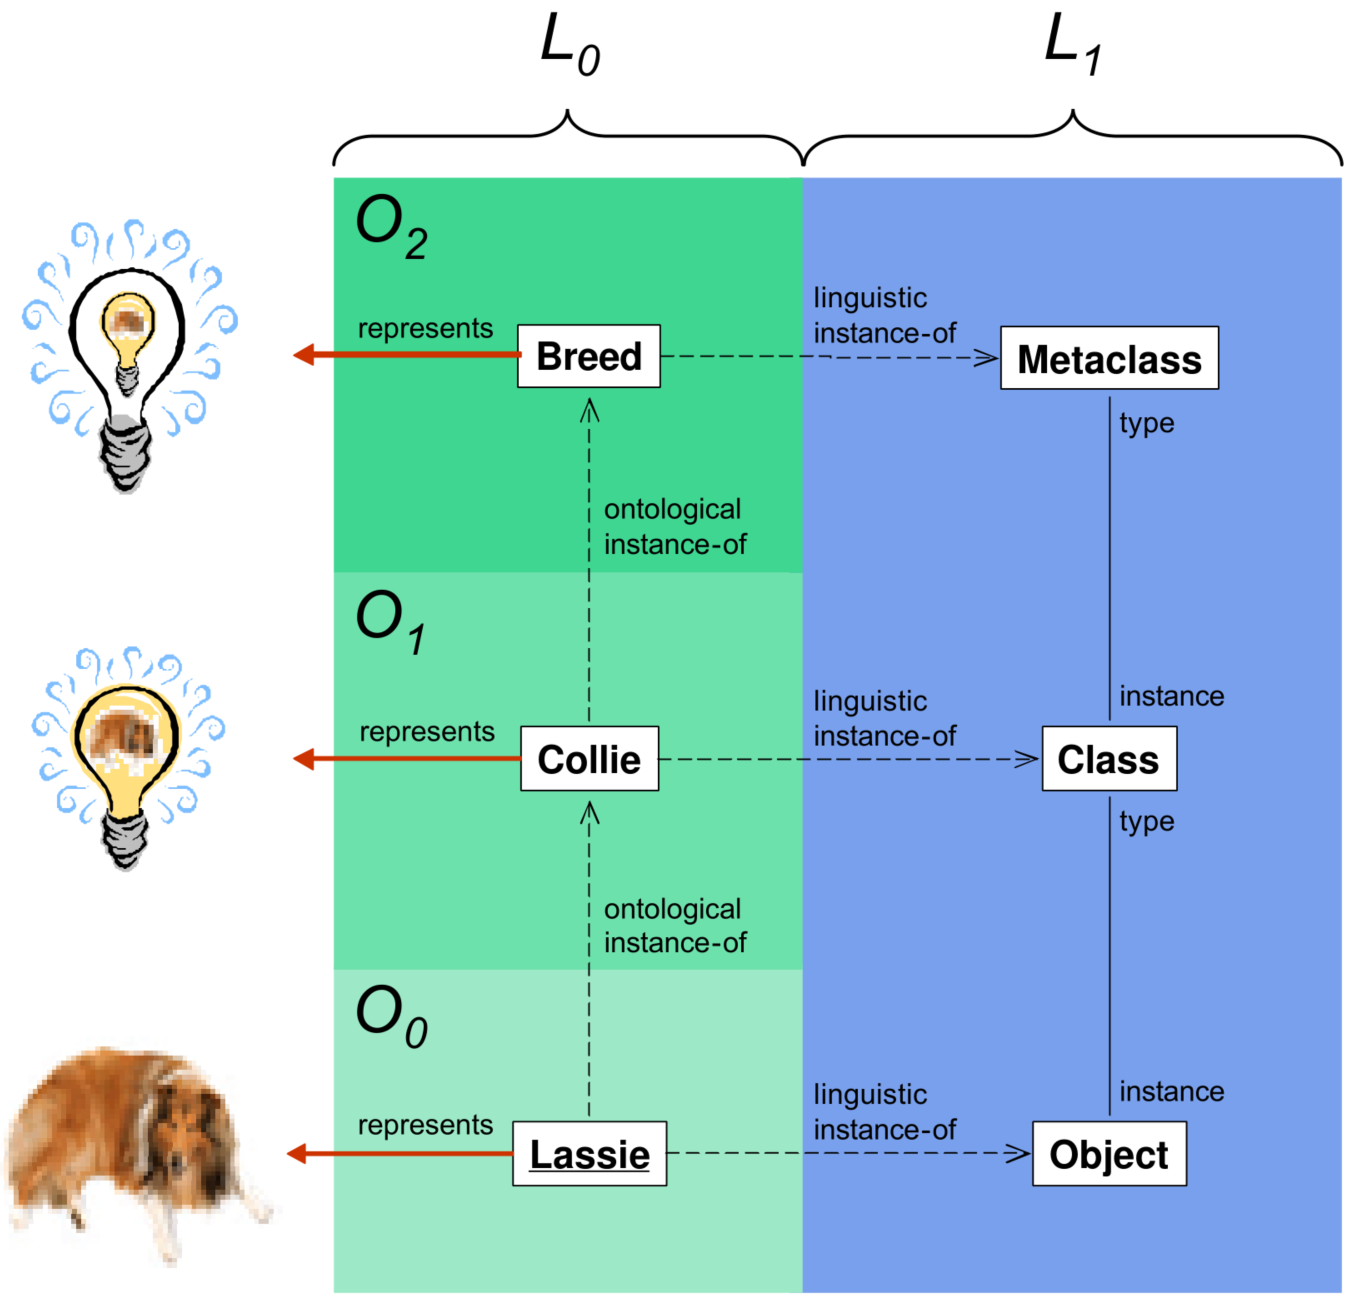
\includegraphics[width=0.4\textwidth]{ontologicalView.png}
			\attribution{C. Atkinson, Th. Kuhne, Model-driven development: a metamodeling foundation, 2003}
		\end{center}
	\end{frame}

	\begin{frame}
		\frametitle{Пример из реальной жизни}
		\begin{center}
			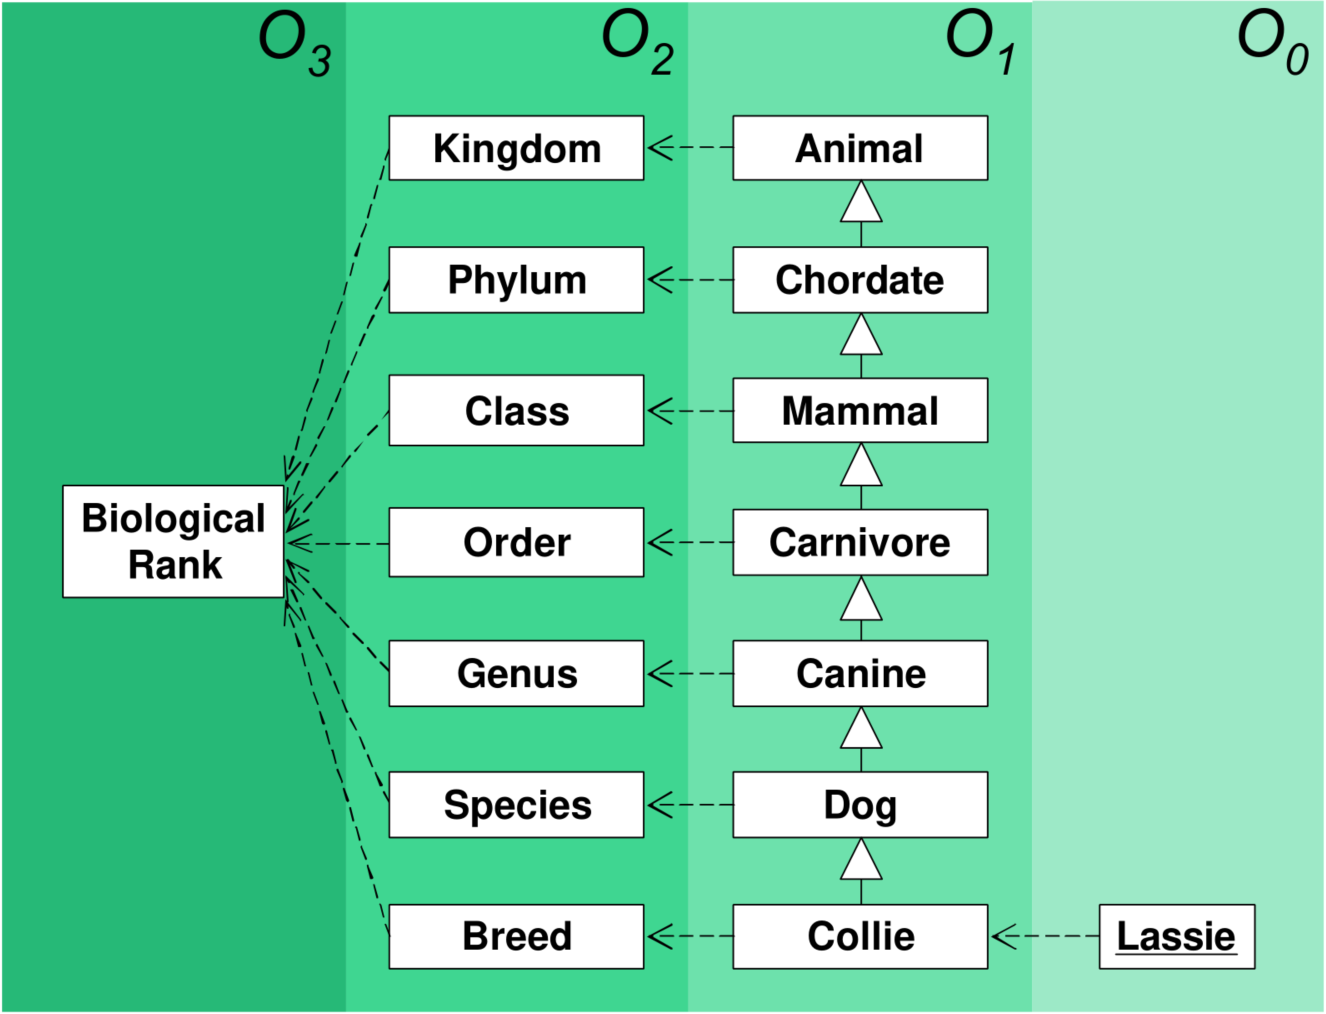
\includegraphics[width=0.6\textwidth]{biologicalClassification.png}
			\attribution{C. Atkinson, Th. Kuhne, Model-driven development: a metamodeling foundation, 2003}
		\end{center}
	\end{frame}

	\section{Существующие реализации}

	\begin{frame}
		\frametitle{Melanee}
		\begin{center}
			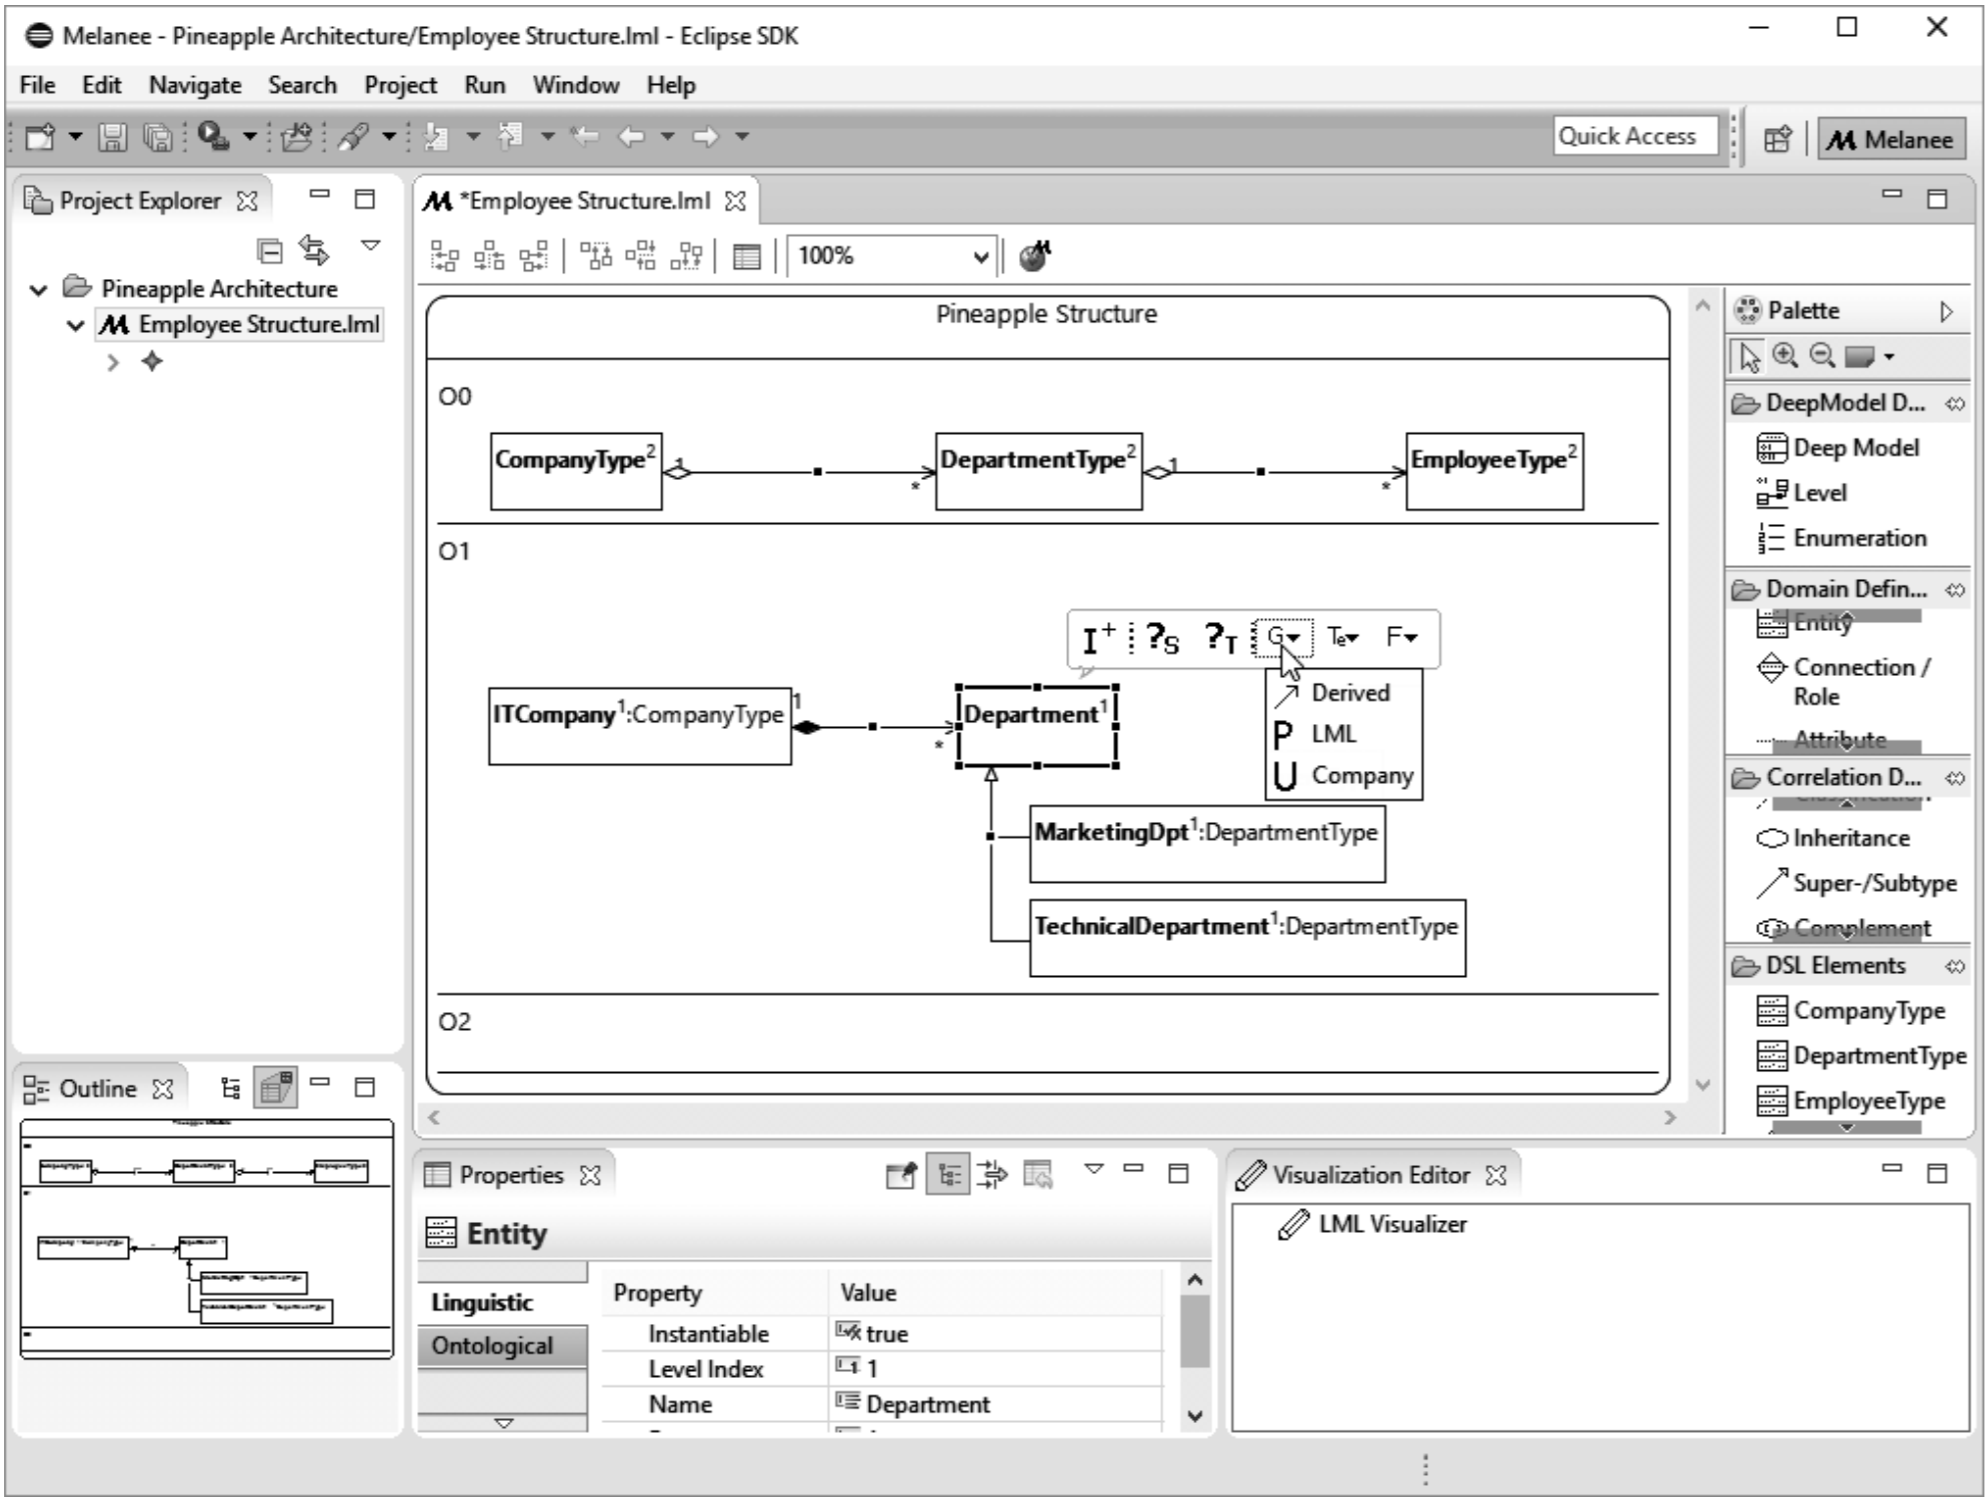
\includegraphics[width=0.75\textwidth]{melanee.png}
			\attribution{C. Atkinson, R. Gerbig,Flexible Deep Modeling with Melanee, 2016}
		\end{center}
	\end{frame}

	\begin{frame}
		\frametitle{WebDPF}
		\begin{center}
			\includegraphics[width=0.75\textwidth]{webDpf.png}
			\attribution{F. Rabbi et al. WebDPF: A web-based metamodelling and model transformation environment, 2016}
		\end{center}
	\end{frame}

	\begin{frame}
		\frametitle{REAL.NET}
		\begin{center}
			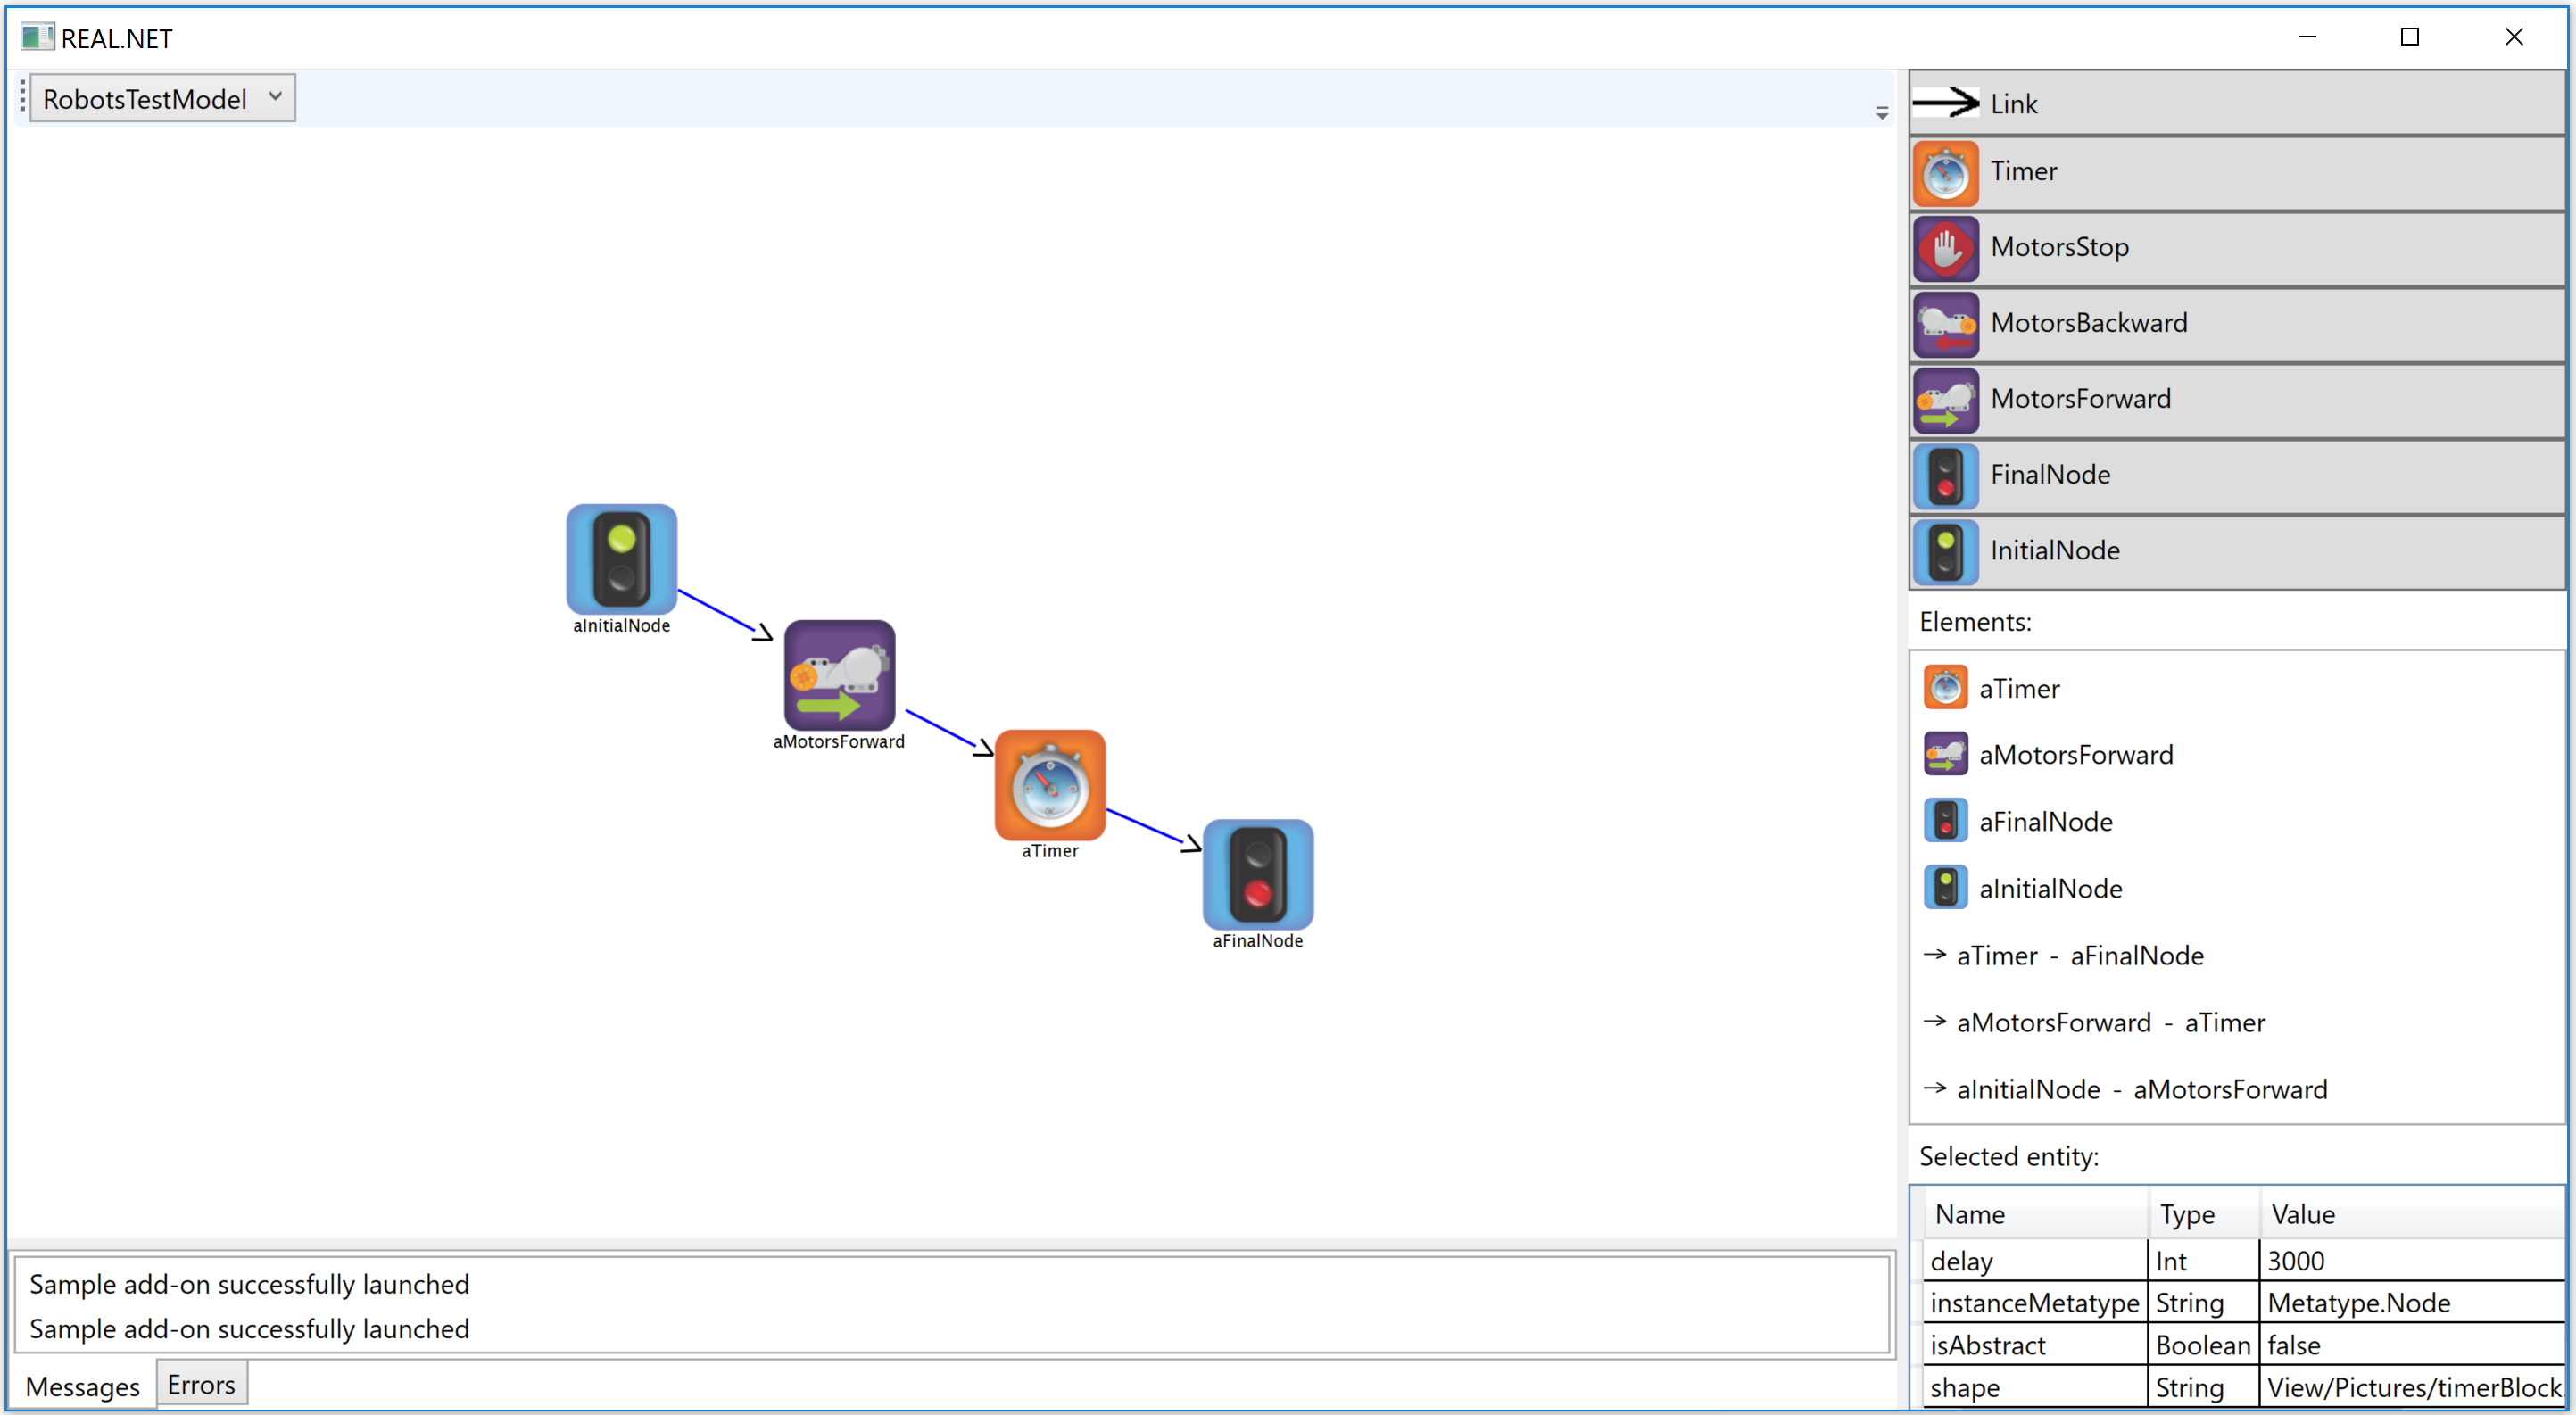
\includegraphics[width=0.95\textwidth]{realNet.png}
		\end{center}
	\end{frame}

	\begin{frame}
		\frametitle{Корневая метамодель REAL.NET}
		\begin{center}
			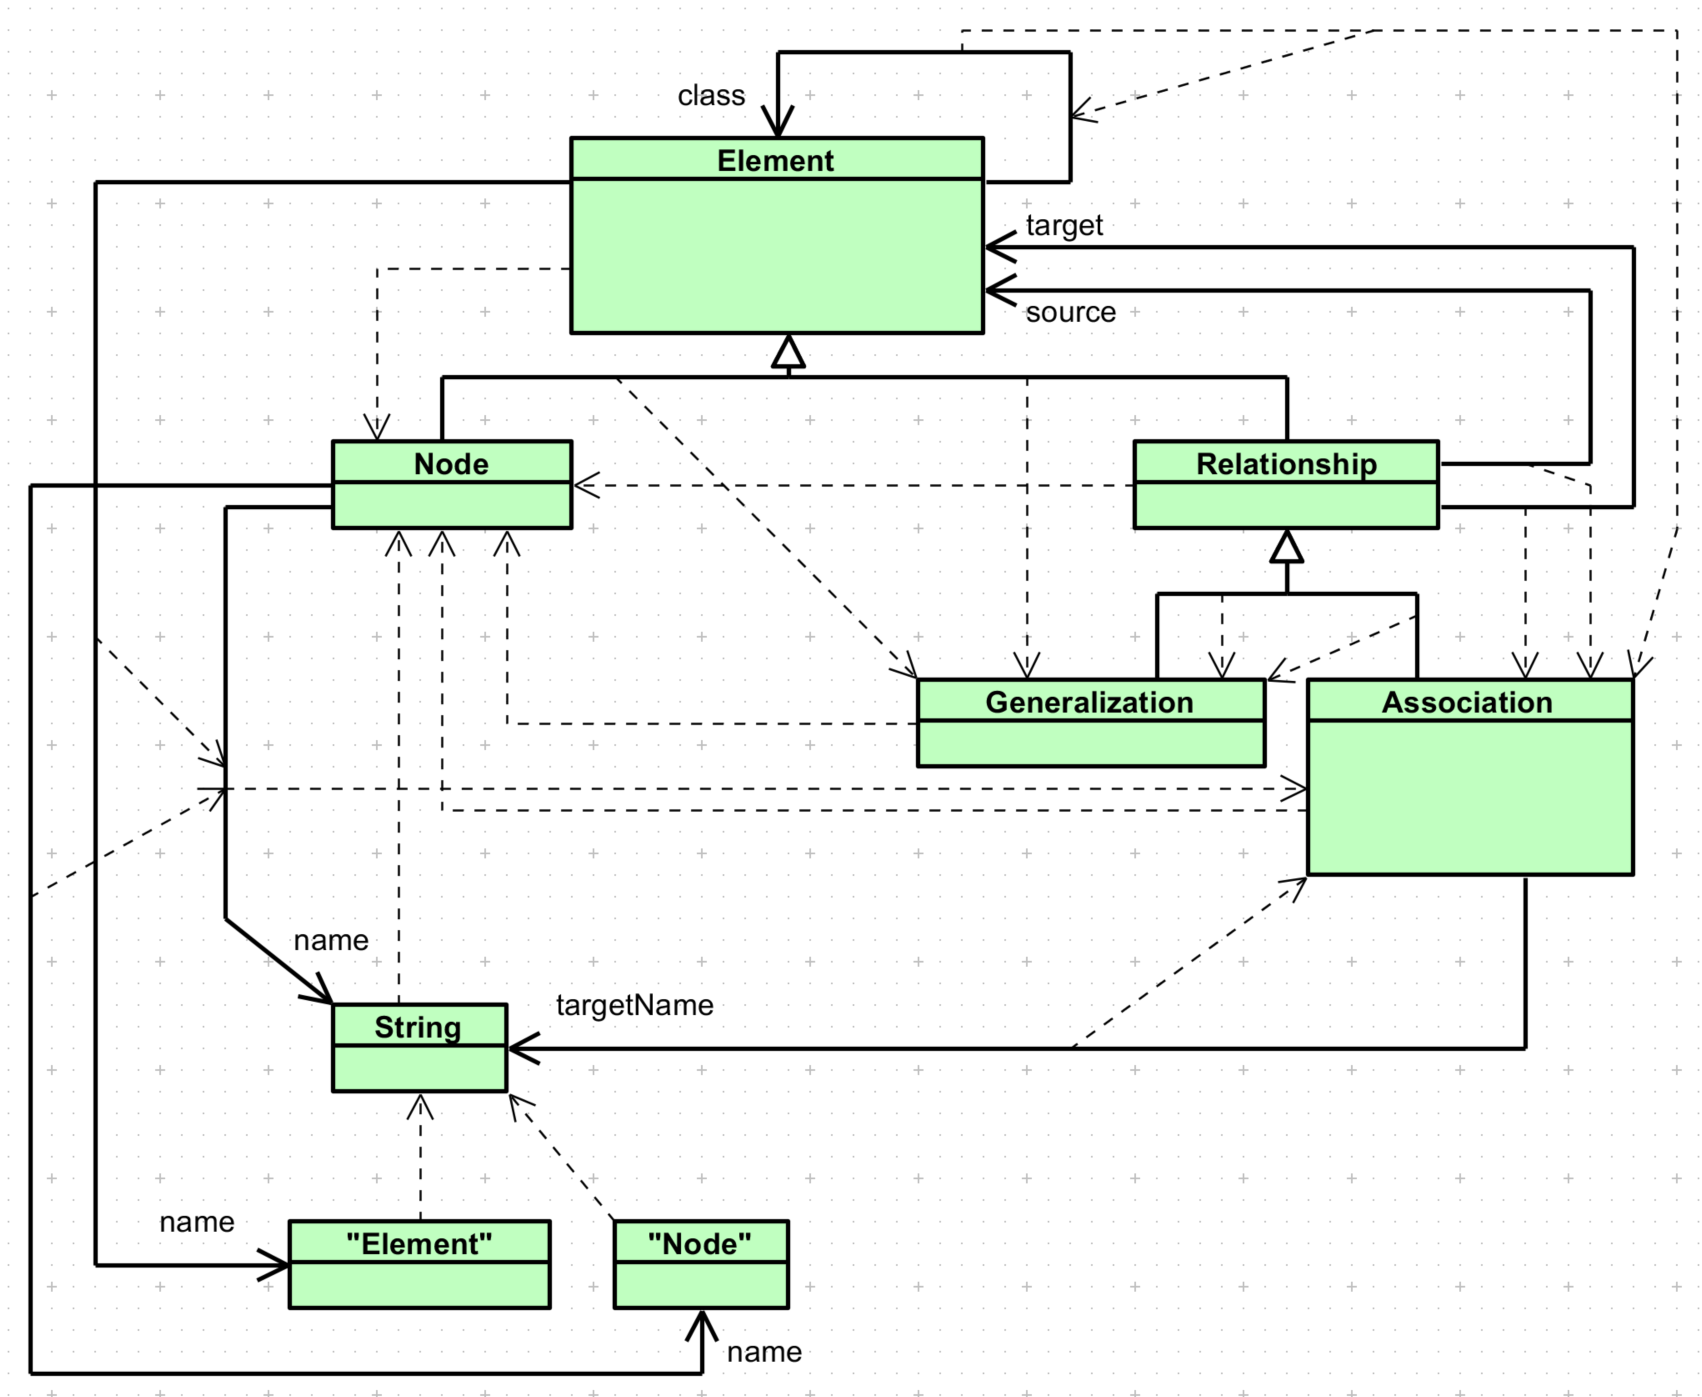
\includegraphics[width=0.65\textwidth]{realNetMetametamodel.png}
		\end{center}
	\end{frame}

	\section{Заключение}

	\begin{frame}
		\frametitle{Заключение}
		\begin{itemize}
			\item UML 2.0, вышедший в 2005 году, придерживается четырёхуровневой схемы, как и UML 2.5.1
			\item Реализации глубокого метамоделирования начали появляться только в 2010-х, далеки от внедрения
			\begin{itemize}
				\item MetaDepth, текстовая среда моделирования от авторов $AToM^3$
			\end{itemize}
			\item Есть и другие интересные подходы, например, Powertypes
		\end{itemize}
	\end{frame}

\end{document}

